\documentclass[onecolumn, draftclsnofoot,10pt, compsoc]{IEEEtran}
\usepackage{graphicx}
\usepackage{url}
\usepackage{setspace}

\usepackage{geometry}
\geometry{textheight=9.5in, textwidth=7in}

% 1. Fill in these details
\def \CapstoneTeamName{		Gesture Recognition}
\def \CapstoneTeamNumber{		33}
\def \GroupMemberOne{			Jonathan Hull}
\def \GroupMemberTwo{			Nicholas Davies}
\def \GroupMemberThree{			Shane Clancy}
\def \GroupMemberFour{          Shihao Song}
\def \GroupMemberFive{          Ulises Zaragoza}
\def \GroupMemberSix{           Zhidong Zhang}
\def \CapstoneProjectName{		Gesture Recognition using new Intel Real Sense light coded Camera}
\def \CapstoneSponsorCompany{ Intel}
\def \CapstoneSponsorPersonOne{		Eduardo X. Alban}
\def \CapstoneSponsorPersonTwo{        Satoshi Suzuki}
\def \CapstoneSponsorPersonThree{        Po-Cheng Chen}

% 2. Uncomment the appropriate line below so that the document type works
\def \DocType{	%Problem Statement
				Requirements Document
				%Technology Review
				%Design Document
				%Progress Report
				}
			
\newcommand{\NameSigPair}[1]{\par
\makebox[2.75in][r]{#1} \hfil 	\makebox[3.25in]{\makebox[2.25in]{\hrulefill} \hfill		\makebox[.75in]{\hrulefill}}
\par\vspace{-12pt} \textit{\tiny\noindent
\makebox[2.75in]{} \hfil		\makebox[3.25in]{\makebox[2.25in][r]{Signature} \hfill	\makebox[.75in][r]{Date}}}}
% 3. If the document is not to be signed, uncomment the RENEWcommand below
%\renewcommand{\NameSigPair}[1]{#1}

%%%%%%%%%%%%%%%%%%%%%%%%%%%%%%%%%%%%%%%
\begin{document}
\begin{titlepage}
    \pagenumbering{gobble}
    \begin{singlespace}
    	%\includegraphics[height=4cm]{coe_v_spot1}
        \hfill 
        % 4. If you have a logo, use this includegraphics command to put it on the coversheet.
        %\includegraphics[height=4cm]{CompanyLogo}   
        \par\vspace{.2in}
        \centering
        \scshape{
            \huge CS Capstone \DocType \par
            {\large\today}\par
            \vspace{.5in}
            \textbf{\Huge\CapstoneProjectName}\par
            \vfill
            {\large Prepared for}\par
            \Huge \CapstoneSponsorCompany\par
            \vspace{5pt}
            {\Large\NameSigPair{\CapstoneSponsorPersonOne}\par}
            {\Large\NameSigPair{\CapstoneSponsorPersonTwo}\par}
            {\Large\NameSigPair{\CapstoneSponsorPersonThree}\par}
            {\large Prepared by }\par
            Group\CapstoneTeamNumber\par
            % 5. comment out the line below this one if you do not wish to name your team
            \CapstoneTeamName\par 
            \vspace{5pt}
            {\Large
                \NameSigPair{\GroupMemberOne}\par
                \NameSigPair{\GroupMemberTwo}\par
                \NameSigPair{\GroupMemberThree}\par
                \NameSigPair{\GroupMemberFour}\par
                \NameSigPair{\GroupMemberFive}\par
                \NameSigPair{\GroupMemberSix}\par
            }
            \vspace{20pt}
        }
        \begin{abstract}
        % 6. Fill in your abstract    
        	Our group’s chosen project for the quarter is the ‘\textit{Gesture Recognition using new Intel RealSense coded light camera}’, and our group consists of the following individuals: Shane Clancy, Nicholas Davies, Jonathan Hull, Shihao Song, Zhidong Zhang and Ulises Zaragoza. This requirements document aims to outline the system requirements of the project and go into detail of how we are expected to verify different project components. We will go into detail about the functionality of the Intel RealSense camera, machine learning model, and graphical user interface, as well as outline the performance requirements for the machine learning model and the graphical user interface. We will also cover the system interface, environmental conditions, information management, policies and regulations, and packaging, handling, shipping, and transportation. Verification of each of these requirements will also be discussed.
        \end{abstract}     
    \end{singlespace}
\end{titlepage}
\newpage
\pagenumbering{arabic}
\tableofcontents
% 7. uncomment this (if applicable). Consider adding a page break.
%\listoffigures
%\listoftables
\clearpage

% 8. now you write!
\section{Introduction}

\subsection{System Purpose}
Our team will collaboratively work to create and train a machine learning (ML) algorithm with the task of gesture recognition using the Intel RealSense Depth Camera SR305. 
In addition our goal is to build a Graphical User Interace (GUI) application to house the model and utilize it.
We will begin with the task of classifying simple gestures such as hand motions (e.g. waving, alphabet sign language, rock, paper, scissors).
The ultimate goal, however, will be to create a sign-language to text classifier to aid those with communication challenges.

\subsection{System Scope}
The system scope of our project has an end goal of having a ML be able to classify sign-language gestures, and present this classification via a text message to the user through the housing GUI application. This GUI application will allow interface capabilities with the RealSense camera, and will be a direct source of input to the ML model. Our project will take on a much smaller initial scope, as we seek to first build and train a foundation ML model that can perform basic gesture recogntion tasks. Once this has been established, we will work to fine-tune the model and prepare it to handle our end-goal task of sign-language recognition.

\subsection{System Overview}

\subsubsection{System Context}
The camera we will be using is the Intel RealSense Depth Camera SR305.
This indoor camera has an incredible quality of depth, specifically when used at the ideal one meter distance.
The code written for this device is easily transferred to utilize on other Intel RealSense gadgets, making it user friendly. 
This camera is also very cost effective, making the product affordable for a wider range of customers.
\\
\\
ML Algorithms are a branch of artificial intelligence that allows computers to learn for themselves. 
ML Algorithms can be supervised or not, allowing them to learn for themselves or have strict guidance depending on the application. 
In this context, our ML Algorithm is going to learn to recognize patterns through visual recognition and coded light in the training videos that we provide.
This will then allow the system to classify new video feeds. 
\\
\\
Coded light systems, a tool utilized by RealSense cameras, interpret the depth and distance by using infrared light.
The infrared light is a single pixel that is cast onto the object to see if the pixel lands on a dark or light stripe.
Then, a binary code is created for each pixel.
This data is then recorded and memorized on the device to help it interpret certain gestures.
The Intel RealSense Depth Camera SR305 has a 640x480 depth resolution as well as 60 frames per second, making for quality video capturing capabilities\cite{first}.

\subsubsection{System Functions}
Our team will be utilizing the SDK provided by Intel on GitHub which will allow us to interface with the camera and use the camera’s features. 
The way we will be implementing our ML Algorithm is through transfer learning approach which is using a pre-trained ML Algorithm as baseline classifier, and will then train the task of gesture recognition from this foundation. 
\subsubsection{User Characteristics}
The individuals we are targeting with this software are those with language barriers. Our goal is to make a software that allows language-disabled people to communicate smoothly with the movement of their hands. We hope to tackle the barrier of interpreting sign language for those not familiar with the gestures, and furthermore to achieve the goal of helping people with language disabilities communicate with the outside world.



\section{System Requirements}

\subsection{Functional Requirements}
The following sections outline the functional requirements that this project needs to meet. We will also evaluate how we will measure these functional requirements in order to meet the needs and expectations of the clients. We will be measuring the functionality of the Intel RealSense camera, machine learning model, and the Graphical User Interface.

\subsubsection{Intel RealSense Camera}
The Intel RealSense camera is a light coded camera that we will be using the capture data for our project. The software for this component has already been developed in an open source environment by Intel. The camera needs to be attached to the computer through USB 3.1, then the Intel RealSense SDK 2.0 has the capability to find and read input of the Intel RealSense camera itself. Our project repository will always include the proper SDK that is compatible with the Intel RealSense SR305 Camera. We will be measuring the functionality by making sure that the depth of certain objects is measured correctly through manual measurements.

\subsubsection{Machine Learning Model}
The machine learning model is the brain of the project, and will need to interact with the Intel RealSense camera, as well as the GUI application. We will be doing our development for the machine learning model using Python3, which needs to be installed in order for the model to be able to train and classify information that is provided to it through the database that we will setup to store our information. Measuring the functionality of the machine learning model will be done after the model is developed and trained. We hope to achieve high accuracy with our model, and we will be measuring its accuracy throughout the development on a set of data that we set aside for testing.

\subsubsection{Graphical User Interface}
The graphical user interface will be in the form of an executable that should be deployable on all platforms. We will need to make sure that this application can be deployed on each platform before we release the project. The user interface needs to be accessible to people who lack verbal communication, and customizable to their needs. Consistent manual testing on the interface needs to be done to ensure the usability meets these standards.

\subsection{Performance Requirements}
The following sections outline the speculative performance requirements for our project’s chosen ML Model and the GUI application our team will create to house and utilize the model. See the Verification section for information on how our group will ensure performance criteria is met.
\subsubsection{Machine Learning Model}
Considering the scope of our project, our ML model will take on two phases of performance requirements. The initial phase will be instantiated for the introductory task we are assigning to our model. The introductory task assigned to our model, is a basic gesture recognition task. This initial phase will require that our model be able to perform basic recognition through the form of video feed provided by the RealSense camera. Examples of basic recognition tasks we expect for our model during the initial phase include less complex hand gestures such as the common game, rock, paper, scissors, or even something as simple as a “peace” sign. The goal with setting this initial phase requirement for our model is to establish a foundation for our model. We then hope to build from this foundation, and train our model to accomplish the higher complexity gesture recognition task of detecting American Sign Language, and will then instantiate phase 2 model performance requirements.
\newline \newline
Phase 2 requirements for our ML model will take the form of enhanced phase 1 requirements, except by this time we will have been training our model on American Sign Language training sets so we will expect our model to be able to accomplish the more complex task of Sign Language gesture recognition. Further specifications have yet to be defined, establishing the kinds of prioritization that will take place in the task of recognizing Sign Language. Further details will be discussed between clients and group members to cement prioritization guidelines within the domain of Sign Language. We will use this guideline to direct the phase 2 requirements for our model.
\newline

\subsubsection{Graphical User Interface}
The performance requirements expected of our GUI include the ability to securely transfer RealSense video feed output as input to the ML model of our project. Our encasing GUI must be able to securely and dependably read input from the RealSense camera, without communication issues between the software and hardware. Furthermore, it is expected that our model's classification is output in a reasonably quick manner. Exact time specifications may be detailed upon deeper experimentation with RealSense cameras and related SDK’s.
\subsection{System Interface}
The interface of our project will come solely through user interaction with the GUI. Specific GUI details have yet to be established, however high level topics needing inclusion have been established by our group. One specific high level need for our GUI will be the requirement that a user may interact with the software with either a keyboard or a mouse, and must not be constrained to one or the other. We hope to include greater accommodation strategies in the future, but our strict requirement of at least those input domains will be an up front expectation for our group. Furthermore, our group will aim to make a user friendly application, that does not overwhelm the user with complex design interfaces. With these two high level specifications set in place, our group has a lot of room to build a solid GUI application around these principles.

\subsection{Environmental Conditions}
The GUI Environment should be on the development machine the client chooses. If no machine is given, then the development location is subject to change. The GUI should be able to run on Windows 10, IOS, and Linux. The environment on which it runs should have internet access and enough processing power in order to properly run all system components and program requirements. 


\subsection{Information Management}
The information most pertinent to our group’s project is the training data we will use as input for our chosen ML model. The management of this data will involve identifying a candidate storage method followed by beginning the process of collecting videos to use as training/test/validation input for our ML model. Due to the high importance of obtaining plentiful and quality forms of training data, the process of collecting data itself will also take on a form of management. This form will involve a strict set of guidelines detailing which types of gestures we are obtaining, length of videos, number of different gesture iterations, involving diverse participants, and potentially other rules yet to be determined. Furthermore, a timeline will be imposed on a data set quantity fulfilment, guaranteeing an adequate amount of data to be readily available for group, whenever we are able to begin training our selected model. These steps must be established and enacted in order for proper execution of our project and relevant goals. 
\subsection{Policies and Regulations}
For work completion, all group members are in accordance  with the given work assigned. If the work completed is code-based, then a peer-review has to be completed prior to submission. If the work completed is text-based, then at least two other group members have reviewed the document. Each process should establish an outline at the beginning and the task should meet all requirements specified by the outline. Work should sufficiently accomplish task at hand. Work should be well thought out with clearly fleshed out ideas. Meeting attendance, is required for every group  member unless properly communicated, or unforeseen circumstances occur. If we encounter problems, it is best to solve them internally. If we can't solve them, then we will escalate as needed.
\subsection{Packaging, handling, shipping, and transportation}
The cameras were initially sent to one group member's home and have been secured. We have divided the cameras amongst the team members, and plan to give equal access throughout the first term so we may all familiarize ourselve with the equipment. Once our project progresses, we will have a better idea on who should hold what equipment at what time(s).
\section{Verification}

\subsection{Functional Requirements}
The following sections outline the verification techniques our group will act on in order to make sure all components of the project are functional.

\subsubsection{Intel RealSense Camera}
The camera needs to cover many edge cases that could be encountered based on the depth calculations and bad IR sensor data. Although the product has been thoroughly tested by Intel, we will need to make sure that the camera can obtain edge case data for certain gestures that we want to classify. While our group is gathering data, we hope to find new edge cases to explore with the camera. This will help the accuracy and training of the machine learning model directly. 

\subsubsection{Machine Learning Model}
The machine learning model will need to be regularly tested in different ways. Once a model is built, we will verify feature importance and relevance, feature thresholds, and feature relationship with output. Some features might not be relevant to classifier, and can be pruned accordingly to increase speed of training and advancement of the model. Feature thresholds are bounds for specific features, and if features can specifically fall within a range, this can be analyzed and a multi-layer model can be developed in order to account for these ranges relating to specific output that is wanted. As a group we will need to continually verify that features are being given different priorities in order to create an accurate model.

\subsubsection{Graphical User Interface}
The graphical user interface needs to go through manual testing, by many different people. This will make sure that the user interface is intuitive and usable by different types of people with different goals for the program. The user interface needs to be customizable to different needs, and any specific need that is not met, should be addressed during verification steps of new feature introduction.

\subsection{Performance Requirements}
The following sections outline the speculative verification techniques/guidelines our group will implement in order to ensure the validity of the performance requirements established above.

\subsubsection{Machine Learning Model}
An essential aspect of this project is the validity of our classification algorithm, and the metrics by which we measure the accuracy of our model. As noted in Aditya Mishra’s article, \textit{Metrics to Evaluate your Machine Learning Algorithm}, there exist multiple methods to evaluate the performance of a ML algorithm. One important note mentioned in Mishra’s article, is how model performance may be viewed differently dependent upon the measuring method used. Mishra then elaborates on several of the different ML accuracy measurement techniques. Each technique highlights different metrics that are used to calculate a score that represents a form of accuracy\cite{second}. Dependent upon the type of ML algorithm our group chooses to implement, we will have to research which evaluation technique best represents the definition of accuracy that we define for our model.

\subsubsection{Graphical User Interface}
The main form of verification for performance of the GUI application, which houses the ML model, will come through various forms of testing of the application. Usability testing, unit testing, regression testing, and other forms, will be utilized on our GUI application to ensure its quality in performance and functionality. Furthermore, this will help our group ensure that proper communication is occurring through our entire project’s pipeline. Starting from the input received by the camera, followed by assurance that the RealSense video feed is being properly fed into our ML algorithm. Lastly, tests will help ensure that the output being displayed by the GUI is true to the output produced by the ML model. The various forms of testing conducted by our group on the housing GUI application will aid in ensuring the performance quality of the entire project, not just solely the GUI application.
\subsection{System Interface}
Users will be able to consistently open the GUI application to interact with the RealSense camera, and the housed ML model. Apart from the rigorous manual testing our group will perform for verification of performance and functional requirements, specifical manual tests will be performed to ensure the quality of the usability for our GUI application. We will be looking to establish metrics such as ease of use, and specifically we hope to address issues that could arise for users with specific accomodation needs.
\subsection{Environmental Conditions}
The system interface should be able to run on popular operating systems.  Anything from Windows 10, IOS, and Linux.  The focus will be on whatever development machine we are tasked with building this on.  The machine will need Internet connection, ports to connect to the camera, processing power to run the machine learning model, and access the database.  The interface can also be made to be portable such as exporting it to a Raspberry Pi or Arduino to run if the group decides that this is its end state.  The database will need to have an adequate amount of space to store training videos.  It is important that the computer running this interface is not hindered by its processing power to avoid unnecessary delays.

\subsection{Information Management}
Ensuring quality and an adequate quantity of training data is vital to the success of our group’s project. Therefore, a formal team meeting needs to take place in order to detail the guideline set and timeline for our project’s data goals. Furthermore, a form of data storage needs to be decided amongst our group members and clients, with the idea in mind that we are going to potentially need a large storage room to store videos as our training/test/validation sets. Once this meeting has taken place, along with the specification of guidelines, timelines, and data storage methods, this document may be signed off.

\subsection{Policies and Regulations}
The policies and regulations of this system interface should reflect those of our client and Oregon State University College of Engineering. This project should aim to keep anonymity, as well as privacy of any individuals caught in the camera's lens. Gesture collection should only be used for maintaining the accuracy of the machine learning model and keeping and up to date database. If this project is used commercially, then this section is subject to change for its correct purpose. 

\subsection{Packaging, handling, shipping, and transportation}
The only package-able items for this interface would be the GUI.  The machine learning model and the database can be remotely connected to.  The could should either be able to be zipped up or tarred to another machine that can access the machine learning model and the database.  Transportation may vary from email, cloud drives, or any sort of transferring service.  Shipping is not applicable to software unless the interface becomes too large to send over the Internet.

\section{Appendices}
\subsection{Assumptions and Dependencies}
\subsubsection{Assumptions}
\begin{itemize}
  \item This document is a fluid requirements list created by the group members in collaboration with the project clients. Future meetings and work will help cement details within this document that reflect the needs of both the group and the client. This document is subject to change.
\end{itemize}
\subsubsection{Dependencies}
\begin{itemize}
  \item The Intel RealSense SDK will be used by our group to interface with the camera and receive video feed\cite{third}.
\end{itemize}
\subsection{Acronyms and Abbreviations}
\begin{itemize}
  \item SDK: Software Development Kit
  \item ML: Machine Learning
  \item GUI: Graphical User Interface
  \item CNN: Convolutional Neural Network
\end{itemize}
\subsection{Gantt Chart Timeline}
Figure 1 below details the tentative timeline for group's projected milestones. 
This timeline currently displays only high level goals and is anticipated to change once finer project details have been firmly established. 
\begin{figure}[htp]
    \centering
    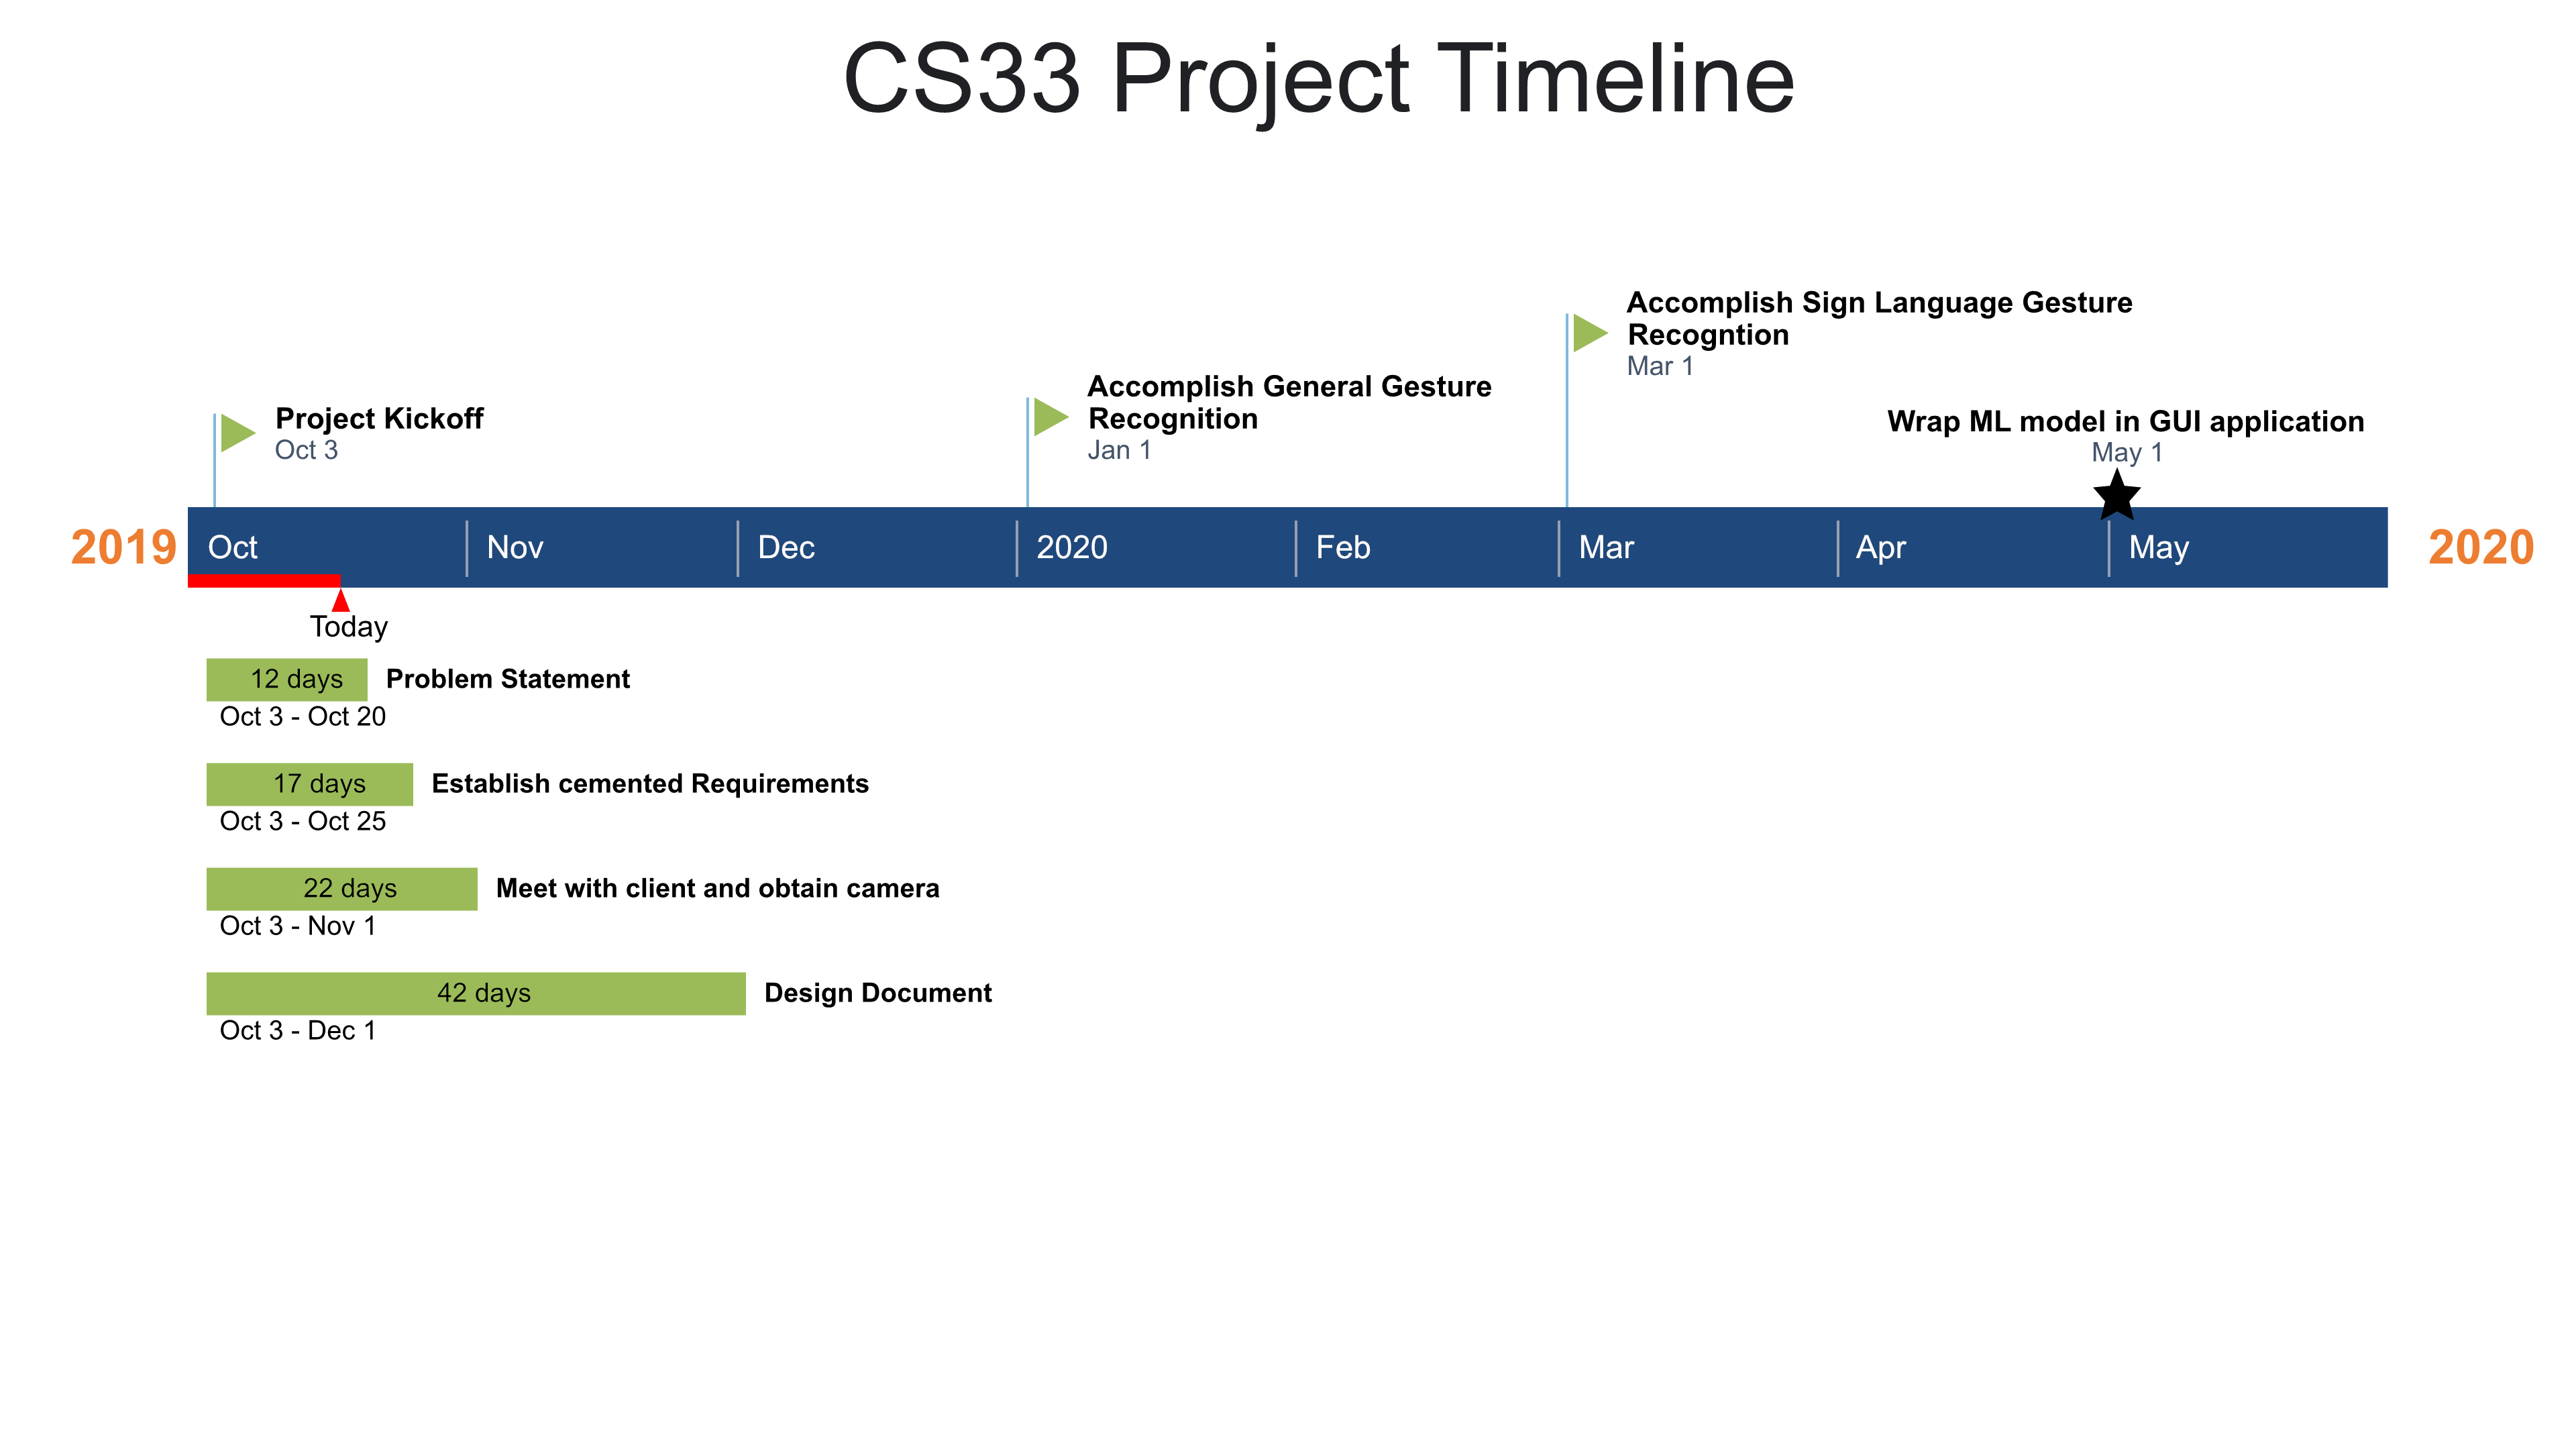
\includegraphics[width=17cm]{SoftwareDevelopment.png}
    \caption{Gantt Chart}
    \label{fig:Gantt Chart}
\end{figure}
\newpage
\begin{thebibliography}{9}

\bibitem{first} 
Intel. 
\textit{Intel® RealSense™ Depth Camera SR305}. 
Intel, 2019. Retrieved on October 15, 2019 from https://www.intelrealsense.com/depth-camera-sr305/.

\bibitem{second} 
Mishra, A. 
\textit{Metrics to Evaluate your Machine Learning Algorithm}. 
Towards Data Science, 2018. Retrieved on October 11, 2019 from https://towardsdatascience.com/metrics-to-evaluate-your-machine-learning-algorithm-f10ba6e38234.


\bibitem{third} 
Intel. 
\textit{Intel® RealSense™ SDK}. 
Intel, 2019. Retrieved on October 11, 2019 from https://github.com/IntelRealSense/librealsense.


\end{thebibliography}
\end{document}